\documentclass[12pt,a4paper]{article}

% ----------------------------
% Packages
% ----------------------------
\usepackage[margin=1in]{geometry}
\usepackage{setspace}
\usepackage{graphicx}
\usepackage{hyperref}
\usepackage{titlesec}
\usepackage{fancyhdr}
\usepackage{datetime2}
\usepackage{float}
\usepackage{adjustbox}
\usepackage{rotating}
\usepackage{acronym} 
\usepackage{subcaption}
\usepackage{graphicx}

% ----------------------------
% Formatting
% ----------------------------
\setstretch{1.2}
\setlength{\parskip}{0.6em}
\setlength{\parindent}{0pt}

\titleformat{\section}
  {\normalfont\Large\bfseries}
  {\thesection}{1em}{}

\titleformat{\subsection}
  {\normalfont\large\bfseries}
  {\thesubsection}{1em}{}

% ----------------------------
% Header / Footer
% ----------------------------
\setlength{\headheight}{15pt}  
\pagestyle{fancy}
\fancyhf{}
\fancyhead[L]{Quantum Imaging Project Plan}
\fancyhead[R]{\leftmark}
\fancyfoot[C]{\thepage}

% ----------------------------
% Document Metadata
% ----------------------------
\title{Graduation Internship}
\author{Samer Saftawi}
\date{February 2026}

% ----------------------------
% Document
% ----------------------------
\begin{document}

\begin{titlepage}
\centering

\vspace*{1.5cm}

{\Large\bfseries Project Plan -- Graduation Internship\par}
\vspace{1.2cm}

{\Huge\bfseries Quantum Imaging with Undetected Photons\par}
\vspace{0.4cm}

{\Large
Project: User Interface focusing on enhanced\\
Quantum image processing\par}

\vspace{2.8cm}

{\large
\begin{tabular}{@{}l l@{}}
\textbf{Author:} & Samer Saftawi \\
\textbf{Study program:} & Bachelor Applied Computer Science \\
\textbf{Student number:} & 541642 \\
\end{tabular}
}

\vspace{1.5cm}

{\large
\begin{tabular}{@{}l l@{}}
\textbf{Supervisor:} & Dr. D. Polishchuk \\
\textbf{Study Coach:} & Dr. A. Khan \\
\textbf{Research group:} & Applied Nanotechnology \\
\textbf{Project:} & Quantum Imaging with Undetected Photons \\
\textbf{Institution:} & Saxion University of Applied Sciences \\
\end{tabular}
}

\vfill

{\large
Internship period: 02.02.2026 -- 03.07.2026\\
}

\end{titlepage}

\newpage
% ----------------------------
% Table of Contents
% ----------------------------
\tableofcontents
\newpage

\listoffigures
\newpage

% ----------------------------
% List of Abbreviations
% ----------------------------
\section*{List of Abbreviations}
\markboth{LIST OF ABBREVIATIONS}{List of Abbreviations} 
\begin{acronym}[]
    \acro{GUI}{Graphical User Interface}
    \acro{CMOS}{Complementary Metal-Oxide-Semiconductor}
    \acro{ANT}{Applied Nanotechnology}
    \acro{QIUP}{Quantum Imaging with Undetected Photons}
    \acro{PPLN}{Periodically-Poled Lithium Niobate}
    \acro{SPDC}{Spontaneous Parametric Down-Conversion}
    \acro{FFT}{Fast Fourier Transform}
    \acro{TLC}{Talent \& Learning Center}
    \acro{IDE}{Integrated Development Environment}
    \acro{SDK}{Software Development Kit}
\end{acronym}
\newpage


% ----------------------------
% Section: Introduction
% ----------------------------
\section{Introduction}
This graduation project is conducted from February 2nd, 2026, to July 3rd, 2026, as part of the Bachelor of Applied Computer Science program at Saxion University of Applied Sciences. The primary objective is to develop a robust automation framework and an intuitive \ac{GUI} for the quantum imaging demonstrator shown in Figure~\ref{fig:demonstrator}. By integrating hardware control with image processing, this project aims to enhance the accessibility and visual impact of quantum optical phenomena for educational purposes.

This Project Plan serves as a roadmap for the internship, detailing the technical approach, project management methodology, and expected outcomes.

\subsection{Background Information}
This project is part of the Quantum Delta program, which aims to accelerate quantum technology developments by fostering a collaborative ecosystem.

A primary challenge in this field is the non-intuitive nature of quantum properties such as entanglement and indistinguishability. The demonstrator addresses this by utilizing \ac{QIUP}.

\subsection{The Setup}

\begin{figure}[H]
  \centering
  \begin{subfigure}[b]{1\linewidth}
    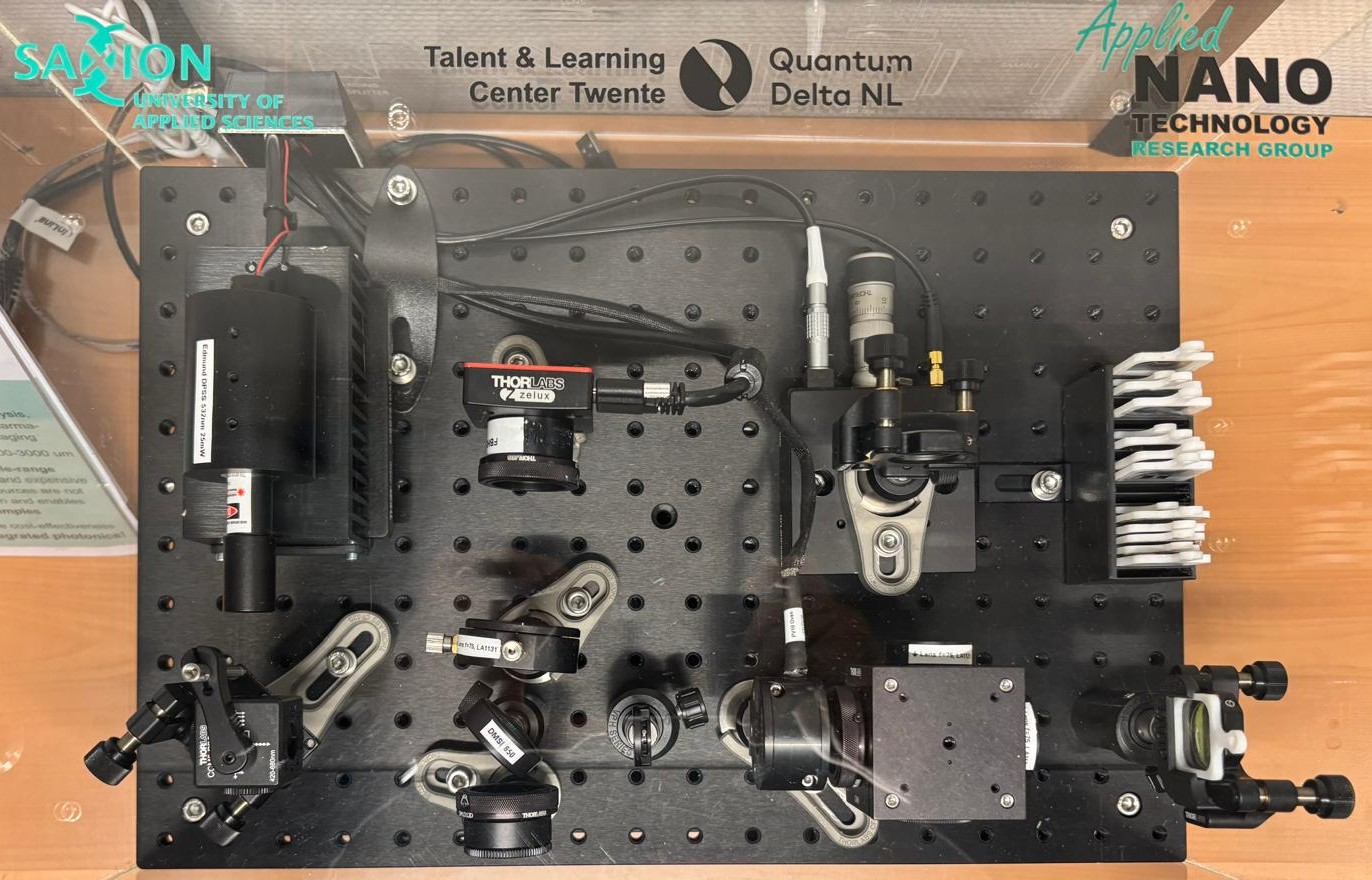
\includegraphics[width=\linewidth]{images/setup/demonstrator_setup.jpeg}
    \caption{Top-Down view on demonstrational setup at Saxion.}
  \end{subfigure}
  \begin{subfigure}[b]{1\linewidth}
    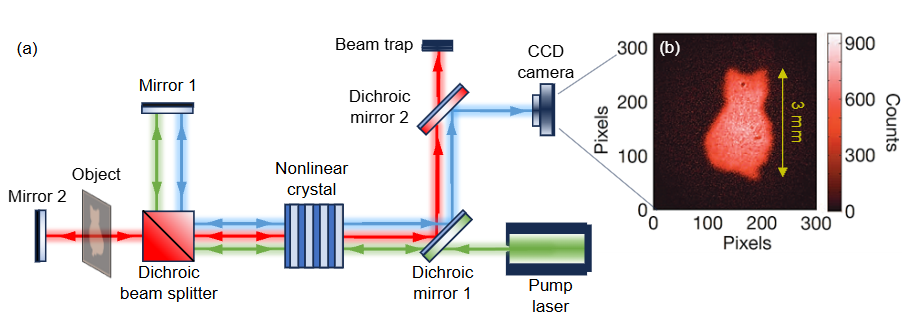
\includegraphics[width=\linewidth]{images/setup/setup_schematic.png}
    \caption{Schematic of demonstrational setups functionality.}
  \end{subfigure}
  \caption{Demonstrational Setup and Schematic.}
  \label{fig:demonstrator}
\end{figure}

The experimental implementation of the quantum imager is shown in Figure \ref{fig:demonstrator}. The system relies on the principle of induced coherence, utilizing a nonlinear interferometer.

As detailed in the schematic (Figure \ref{fig:demonstrator}b), a continuous wave pump laser is directed into a nonlinear crystal specifically, a \ac{PPLN} crystal. Through \ac{SPDC}, the pump photon splits into a signal photon (visible spectrum) and an idler photon (infrared). A dichroic beam splitter separates these paths: the visible signal is reflected by a reference mirror (Mirror 1), while the infrared idler interacts with the target object before being reflected by Mirror 2.

The idler photons that pass through the object contain spatial information about its absorption or phase profile. When the idler and signal beams recombine at the crystal, quantum interference modulates the intensity of the signal beam based on the idler's path information. Consequently, the image of the object which was only "seen" by the infrared light is transferred to the visible spectrum and detected by the CCD camera.

The physical realization of this schematic is shown in Figure \ref{fig:demonstrator}a. The setup is constructed on an optical breadboard to ensure stability. The pump source directs the beam through conditioning optics towards the central crystal mount. The detection module utilizes a Thorlabs Zelux \ac{CMOS} camera to capture the interference patterns. 
\newpage
% ----------------------------
% Section: Assignment Description
% ----------------------------

\section{Assignment Description}
The assignment focuses on transforming a manually controlled demonstrational setup into a robust, automated, and user-friendly demonstrator for \ac{QIUP}. The system currently relies on generic camera software without any image processing.

The work consists of Python-based hardware automation, \ac{FFT}-based image reconstruction, and \ac{GUI} development.

\subsection{Objectives and Student Activities}
\begin{itemize}
    \item \ac{FFT}-based reconstruction of visibility, contrast, and phase images.
    \item Python control of \ac{CMOS} camera and piezoelectric stage.
    \item \ac{GUI} for live acquisition and demonstrator operation.
    \item Automation for stability and repeatability.
    \item Technical documentation and knowledge transfer.
\end{itemize}

\subsection{Deliverables}
\begin{itemize}
    \item Python automation software.
    \item \ac{GUI} (Application/runnable Code -- To Be Determined).
    \item Technical and operational documentation.
    \item Project plan.
    \item Learning report.
    \item Final thesis report.
\end{itemize}

\newpage




% ----------------------------
% Section: Organization
% ----------------------------
\section{Organization -- TODO --}

\subsection{Supervisor \& Study Coach}
The project is supervised by Dr. D. Polishchuk, a senior researcher at \ac{ANT}. Weekly meetings ensure technical alignment and progress monitoring. 

Dr. A. Khan from the Applied Computer Science program will be the study coach.

\subsection{Stakeholders}
The success of this demonstrator project is supported by a collaboration between several key organizations within the Dutch quantum ecosystem.

\begin{itemize}
    \item \textbf{\ac{ANT} Research Group:} As the primary host of the internship, the \ac{ANT} group at Saxion University of Applied Sciences is responsible for the physical development, image processing and scientific validation of the quantum setup.
    \item \textbf{Quantum \ac{TLC} Twente:} 
    \item \textbf{Quantum Delta NL:} 
\end{itemize}

\newpage


% ----------------------------
% Section: Planning
% ----------------------------

\section{Planning}
The project can be divided into 3 main tasks:

\begin{itemize}
    \item \textbf{Documentation:} Code quality, user manuals, and thesis writing.
    \item \textbf{Research:} Quantum optics literature, \ac{FFT} theory, and hardware \ac{SDK} analysis.
    \item \textbf{Implementation:} Python drivers, acquisition synchronization, and \ac{GUI} development.
\end{itemize}

A Gantt chart visualizes a rough project timeline setting milestones and development sprints which is provided in Appendix \ref{appendix:gantt}.

\newpage



% ----------------------------
% Section: Methodology
% ----------------------------
\section{Methodology}

To manage the iterative nature of software development alongside research and hardware integration, this project utilizes Scrum. The Agile approach allows for flexibility in development while ensuring continuous delivery of software features. Figure \ref{fig:scrum_cycle} demonstrates how a Scrum cycle works, visualizing the advantage for iterative progress.

% Diagram of the Scrum process
\begin{figure}[H]
    \centering
    % Placeholder for a Scrum diagram
    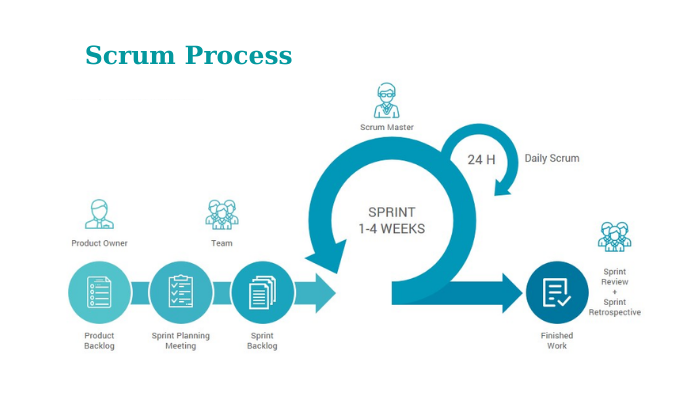
\includegraphics[width=1\linewidth]{images/scrum-cycle.png} 
    \caption{The Scrum Cycle}
    \label{fig:scrum_cycle}
\end{figure}


\subsection{The Sprint Cycle}
The project is divided into weekly sprints. This duration provides a balance between sufficient development time and frequent feedback loops.
At the end of each sprint the past sprint will be reviewed and the next sprint will be adjusted according to past progress. Figure \ref{fig:scrum_cycle} shows the cycle for each sprint.


\subsection{Definition of Done}
To ensure quality and maintainability, a task is only considered "Done" when the following criteria are met:
\begin{enumerate}
    \item The code is written in Python.
    \item The feature is version-controlled and pushed to the repository.
    \item The functionality has been tested on the physical setup.
\end{enumerate}

\subsection{Development Tools}
\begin{itemize}
    \item \textbf{Version Control:} Git and GitHub will be used for source code management.
    \item \textbf{IDE:} Visual Studio Code is the chosen \ac{IDE} for Python development. 
    \item \textbf{Documentation:} LaTeX will be used for all technical documentation and deliverables to ensure professional formatting and visual consistency.
\end{itemize}

\subsection{Communication and Reporting}
To maintain project momentum, the following communication protocols are established:
\begin{itemize}
    \item \textbf{Weekly Stand-ups:} Formal progress review every week to discuss Sprint outcomes and address challenges.
    \item \textbf{Meeting Documentation:} All meeting notes will be published on GitHub.
\end{itemize}


\subsection{Approach \& Strategy}
To achieve the main objective of creating a fully automated \ac{GUI} capable of live quantum image reconstruction, the most promising analysis technique is \ac{FFT}. The implementation will rely on the FFTW library, widely regarded as the industry standard for performance.

To surpass the signal-to-noise limitations of standard single-shot imaging, the experimental setup will  use a piezoelectric stage. This device, mounted on the reference mirror, enables precise control over the optical path length of the interferometer. 

\newpage

% ----------------------------
% Section: Risk Analysis 
% ----------------------------
\section{Risk Analysis \& Achievability}

This section outlines potential obstacles that could impact the project and explains why the assignment remains achievable within the internship period.

\subsection{Potential Risks}
\begin{itemize}
    \item \textbf{Complexity and Misunderstandings}
    The theoretical background of quantum imaging is complex. If the physics are misunderstood, it could lead to incorrect software logic, requiring code to be rewritten later. This could delay sprints. To prevent this, regular alignment meetings with the supervisor will be held to ensure the software strictly follows the physical theory.

    \item \textbf{Hardware Malfunctioning}
    The project relies on specific laboratory equipment like the laser, camera, and crystal which are already present. Since critical components are difficult to replace, a failure would halt data collection. To mitigate this, a lab instruction course will be followed to ensure adherence to standard procedures. Additionally, thorough discussions with the supervisor will clarify operational limitations and potential risks to prevent damage to the setup.

    \item \textbf{Python Support for Hardware}
    The camera and piezoelectric stage may rely on older drivers that do not have native Python support. This could make the initial connection difficult. The mitigation is to audit the drivers in the first week and use wrapper libraries if direct Python support is unavailable.
\end{itemize}

\subsection{Achievability}
Despite the technical risks, this project is highly achievable. The most significant advantage is that the optical setup is already built, calibrated, and physically present, eliminating any delays related to ordering or assembling parts. With the hardware ready and expert supervision available for the physics aspects, the project goals are realistic and attainable within the five-month timeframe.

\section{Appendix}
\appendix
\section{Gantt Chart}
\label{appendix:gantt}

\begin{figure}[H] % [H] forces the image to stay exactly here
    \centering
    \rotatebox{90}{
        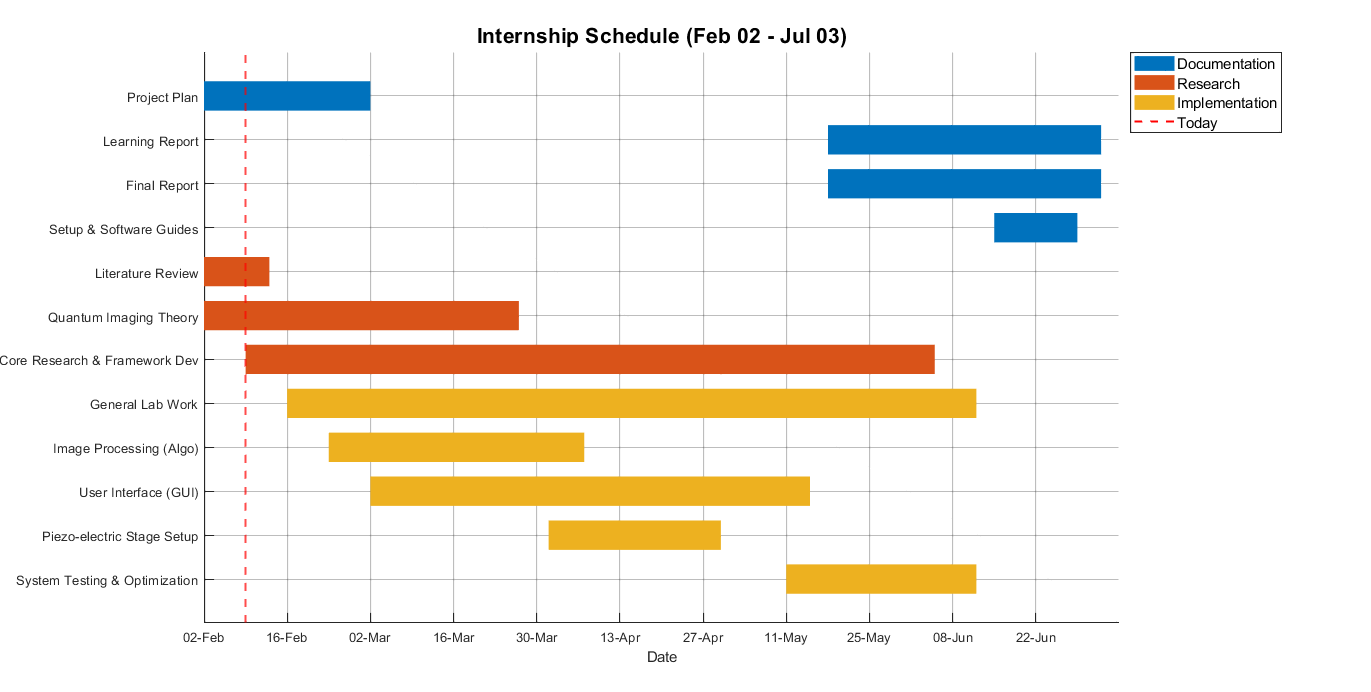
\includegraphics[width=0.85\textheight, keepaspectratio]{images/gantt.png}
    }
    \caption{Planning Timeline -- Gantt Chart}
    \label{fig:gantt}
\end{figure}

\end{document}